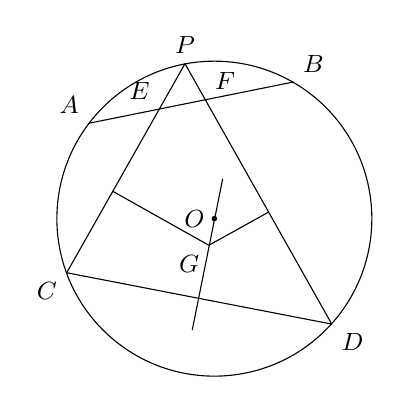
\begin{tikzpicture}[line cap=round,line join=round,font=\small]
% 轮廓及辅助线取固定原 PDF 矢量坐标；交点按直线交点定位。
\draw (0,0) circle (2);
\coordinate (O) at (0,0);
\coordinate (A) at (-1.596,1.211);
\coordinate (B) at (1.002,1.735);
\coordinate (P) at (-0.373,1.968);
\coordinate (C) at (-1.875,-0.687);
\coordinate (D) at (1.491,-1.339);
\coordinate (E) at (intersection of A--B and P--C);
\coordinate (F) at (intersection of A--B and P--D);
\coordinate (G) at (-0.070,-0.338);
\draw (A)--(B) (P)--(C) (P)--(D) (C)--(D);
\draw (0.105,0.501)--(-0.280,-1.409);
\draw (G)--(-1.293,0.349) (G)--(0.687,0.082);
\foreach \pt/\pos in {A/above left,B/above right,C/below left,D/below right,P/above,E/above left,F/above right,O/left,G/below left}{\node[\pos] at (\pt) {$\pt$};}
\fill (O) circle (1pt);
\end{tikzpicture}
